%------------------------------------------------------------------------------
% Template file for the submission of papers to IUCr journals in LaTeX2e
% using the iucr document class
% Copyright 1999-2013 International Union of Crystallography
% Version 1.6 (28 March 2013)
%------------------------------------------------------------------------------

\documentclass[preprint]{iucr}              % DO NOT DELETE THIS LINE
\usepackage{bm}
% \usepackage{graphicx}
% \usepackage{tabularx}
% \usepackage{subfigure}
% \usepackage{afterpage}
% \usepackage{sansmath}
\usepackage{mathtools}
% \usepackage{parskip}
% \usepackage{tikz}
% \usepackage{tikzorbital}
% \usepackage{setspace}
% \usepackage{xcolor}
\usepackage{amssymb}
% \usepackage{bm}
\usepackage{amsmath}
% \usepackage{fancyhdr}
% \usepackage{rotating}
\usepackage{siunitx}
\usepackage[hyphens,spaces,obeyspaces]{url}
\usepackage{color}
\usepackage{siunitx}
\usepackage[hyphens,spaces,obeyspaces]{url}
\usepackage{color}
%\usepackage{cprotect}
\usepackage{textgreek}
\usepackage[normalem]{ulem}
\usepackage{makecell}

\newcommand{\todo}[1]{{\color{red}[TODO: "#1'']}}
\newcommand{\inblue}[1]{{\color{blue}#1}}
\newcommand{\inred}[1]{{\color{red}#1}}
\newcommand{\ingreen}[1]{{\color{green}#1}}



     %-------------------------------------------------------------------------
     % Infobrmation about journal to which submitted
     %-------------------------------------------------------------------------
     \journalcode{S}              % Indicate the journal to which submitted
                                  %   A - Acta Crystallographica Section A
                                  %   B - Acta Crystallographica Section B
                                  %   C - Acta Crystallographica Section C
                                  %   D - Acta Crystallographica Section D
                                  %   E - Acta Crystallographica Section E
                                  %   F - Acta Crystallographica Section F
                                  %   J - Journal of Applied Crystallography
                                  %   M - IUCrJ
                                  %   S - Journal of Synchrotron Radiation

\begin{document}                  % DO NOT DELETE THIS LINE

     %-------------------------------------------------------------------------
     % The introductory (header) part of the paper
     %-------------------------------------------------------------------------

     % The title of the paper. Use \shorttitle to indicate an abbreviated title
     % for use in running heads (you will need to uncomment it).

\title{Calculation of diffraction profiles for perfect crystals obtained as analytical solutions of Takagi-Taupin equations}
% * <msanchezdelrio@gmail.com> 2018-09-25T09:38:50.716Z:
%
% ^.
%\shorttitle{Short Title}

     % Authors' names and addresses. Use \cauthor for the main (contact) author.
     % Use \author for all other authors. Use \aff for authors' affiliations.
     % Use lower-case letters in square brackets to link authors to their
     % affiliations; if there is only one affiliation address, remove the [a].

\cauthor[a]{Jean-Pierre}{Guigay}{guigay@esrf.eu}{address if different from \aff}
\author[a]{Manuel}{Sanchez del Rio}


\aff[a]{European Synchrotron Radiation Facility, 71 Avenue des Martyrs F-38000 Grenoble \country{France}}


     % Use \shortauthor to indicate an abbreviated author list for use in
     % running heads (you will need to uncomment it).

%\shortauthor{Soape, Author and Doe}

     % Use \vita if required to give biographical details (for authors of
     % invited review papers only). Uncomment it.

%\vita{Author's biography}

     % Keywords (required for Journal of Synchrotron Radiation only)
     % Use the \keyword macro for each word or phrase, e.g. 
     % \keyword{X-ray diffraction}\keyword{muscle}

%\keyword{keyword}

     % PDB and NDB reference codes for structures referenced in the article and
     % deposited with the Protein Data Bank and Nucleic Acids Database (Acta
     % Crystallographica Section D). Repeat for each separate structure e.g
     % \PDBref[dethiobiotin synthetase]{1byi} \NDBref[d(G$_4$CGC$_4$)]{ad0002}

%\PDBref[optional name]{refcode}
%\NDBref[optional name]{refcode}

\maketitle                        % DO NOT DELETE THIS LINE

\begin{synopsis}
The Takagi-Taupin equations are solved in its simpler form (zero deformation) and equations of the diffracted and transmitted amplitudes are obtained. Then, the case of a multilayered crystal is discussed using a matrix model. 
\end{synopsis}

\begin{abstract}

The Takagi-Taupin equations are solved in its simpler form (zero deformation) and equations of the diffracted and transmitted amplitudes are obtained. Then, the case of a multilayered crystal is discussed using a matrix model. 

\end{abstract}


     %-------------------------------------------------------------------------
     % The main body of the paper
     %-------------------------------------------------------------------------
     % Now enter the text of the document in multiple \section's, \subsection's
     % and \subsubsection's as required.

\section{Introduction}

The Takagi-Taupin \cite{Takagi1962, Taupin, Taupin1967} equations...

%%%%%%%%%%%%%%%%%%%%%%%%%%%%%%%%%%%%%%%%%%%%%%%%%%%%
%
%%%%%%%%%%%%%%%%%%%%%%%%%%%%%%%%%%%%%%%%%%%%%%%%%%%%
\section{The Takagi-Taupin equations}
\label{sec:TT}

Let us start with the Helmholz equation in a crystal

\begin{equation}
\label{eq:helmholz}
    \Delta \Psi + k^2 (1+\chi) \Psi = 0,
\end{equation}
with $\chi$ the electric susceptibility and $\Psi$ the electric time-independent perturbance. In a crystal, $\chi$ can be expanded in Fourier series,
\begin{equation}
\label{eq:chi}
    \chi = \sum_{\textbf{h}} \chi_h \exp(i \textbf{h} . \textbf{r}),
\end{equation}
where $\bf{h}$ is the reciprocal lattice vector (with modulus $2\pi/d_\text{spacing}$), and the sum goes over all possible reflections (Miller indices $\bf{h}$). When a single reflection $\bf{h}$ is considered, only the terms $\bf{0}$, $\bf{h}$ and $\bf{-h}$ are non-zero, 
\begin{equation}
\label{eq:chisimple}
    \chi = \chi_0 + \chi_{h} \exp(i \textbf{h} . \textbf{r}) + \chi_{-h} \exp(-i \textbf{h} . \textbf{r}).
\end{equation}

The x-ray wavefield inside the crystal is expressed as the sum of two modulated plane waves
\begin{equation}
\label{eq:wavefield}
    \Psi(\textbf r) = D_0(\textbf r) e^{i \textbf k_0 . \textbf r} + D_h(\textbf r) e^{i \textbf k_h . \textbf r},
\end{equation}
with amplitudes $D_{0,h}(\textbf r)$.
% The spatial position $\textbf r$ is expressed in oblique coordinates $(s_0,s_h)$ along the directions of the $\vec k_0$
The vectors $\textbf{k}_0$ and $\textbf k_h=\textbf k_0 + \textbf h$ are the in-vacuum wave-vectors of modulus $k=|\textbf{k}_0|=|\textbf{k}_h|=2\pi/\lambda$, where $\lambda$ is x-ray wavelength. 
% $\textbf{h}$ is the Bragg diffraction vector of the undeformed crystal.

% The Takagi-Taupin equations are obtained 
Inserting the equations~(\ref{eq:chisimple}) and (\ref{eq:wavefield}) in (\ref{eq:helmholz}), and supposing $D_{0,h}$ to be slowly varying amplitudes, thus neglecting the 2$^{\text{nd}}$ order derivatives of $D_{0,h}$,  so that
\begin{equation}
\label{eq:approxslowlyvarying}
(\Delta + k^2)[D_{0,h}(\textbf{r}) \exp(i\textbf{k}_{0,h} . \textbf{r}))] \approx \exp(i\textbf{k}_{0,h} . \textbf{r}) [2 i \textbf{k}_{0,h} . \overset{\rightarrow} \partial D_{0,h} + (k^2 - k^2_{0,h}) D_{0,h}],
\end{equation}
we obtain the Takagi-Taupin equations
\begin{subequations}
\label{eq:TTvector}
\begin{align}
2 i \textbf{k}_0 . \overset{\rightarrow} \partial D_0 + [k^2 - k_0^2 + \chi_0 k^2] D_0 + \chi_{-h} D_h =& 0; \\
2 i \textbf{k}_h . \overset{\rightarrow} \partial D_h + [k^2 - k_h^2 + \chi_0 k^2] D_h + \chi_{h} D_0 =& 0.
\end{align}
\end{subequations}

The spatial position $\textbf r$ is expressed in oblique coordinates $(s_0,s_h)$ along the directions of the $\textbf k_0$ and $\textbf k_h$ (unit vectors $\hat{ \textbf{s}}_{0,h}$). We observe that $d s_0 = \overset{\rightarrow} \partial s_0 . [ d s_0 \hat s_0 + d s_h \hat{\textbf{ s}}_h ]$ implies $\overset{\rightarrow} \partial s_0 . \hat{\textbf{s}}_0=1$ and $\overset{\rightarrow} \partial s_0 . \hat{\textbf{s}}_h=0$. Similarly, $\overset{\rightarrow} \partial s_h . \hat{\textbf{s}}_h=1$ and $\overset{\rightarrow} \partial s_h . \hat{\textbf{s}}_0=0$. For any function $F(s_0,s_h)$ we have 

\begin{subequations}
\label{eq:equalities}
\begin{align}
\hat s_0 \overset{\rightarrow} \partial F=
\hat s_0 \left[ 
\frac{\partial F}{\partial s_0} \overset{\rightarrow} \partial s_0 + 
\frac{\partial F}{\partial s_h} \overset{\rightarrow} \partial s_h \right] 
=& \frac{\partial F}{\partial s_0}
; \\
\hat s_h \overset{\rightarrow} \partial F =& 
\frac{\partial F}{\partial s_h}.
\end{align}
\end{subequations}

\inred{Using $|\textbf k_0| = k = 2 \pi / \lambda$, $k^2 - k_h^2 = \alpha k^2$, being $\alpha$ the deviation of the incident plane-wave $\textbf k_0$ from the Bragg position}

\begin{equation}
\label{eq:alpha}
\alpha = \frac{k^2-(\textbf k_0 + \textbf h)^2}{k^2} = \frac{\textbf h^2 + 2 \textbf k_0 . \textbf h}{k^2} = 4 \sin \theta_B (\sin \theta - \sin \theta_B) \approx 2 (\theta-\theta_B) \sin 2\theta_B),
\end{equation}
where $\theta$ is the glancing angle on the reflective planes, and $\theta_B$ the Bragg angle ($h=2 k \sin\theta_B$, $\textbf k_0 . \textbf h = -2 k \sin\theta$). Note that the last approximation fails far from the Bragg position or if $\cos\theta_B \rightarrow 0$ (normal incidence). 

Using the approximation
\begin{equation}
\label{eq:approxKH}
\textbf k_h . \overset{\rightarrow} \partial D_h = |\textbf k_h| \frac{\partial D_h}{\partial s_h} \approx k \frac{\partial D_h}{ \partial s_h},
\end{equation}
we obtain from equations~(\ref{eq:TTvector})
\begin{subequations}
\label{eq:TT}
\begin{align}
\frac{\partial D_0}{\partial s_0} =& \frac{ik}{2} \left[ \chi_0 D_0(s_0,s_h)+ \chi_{-h} D_h(s_0,s_h) \right]
= i u_0 D_0(s_0,s_h) + i u_{-h} D_h(s_0,s_h); \\
\frac{\partial D_h}{\partial s_h} =& \frac{ik}{2} \left[ (\chi_0 + \alpha) D_h(s_0,s_h)+ \chi_{h} D_0(s_0,s_h) \right] = i (u_0 + \alpha') D_h(s_0,s_h) + i u_{h} D_0(s_0,s_h),
\end{align}
\end{subequations}
where it has been used the notation $u_{0,h,-h}=(\lambda/\pi) \chi_{0,h,-h}$ and $\alpha' = (\lambda/\pi) \alpha$.



%%%%%%%%%%%%%%%%%%%%%%%%%%%%%%%%%%%%%%%%%%%%%%%%%%%%
%
%%%%%%%%%%%%%%%%%%%%%%%%%%%%%%%%%%%%%%%%%%%%%%%%%%%%
\section{Solutions of TT equations for perfect crystals}
\label{sec:TTsolutions}

\subsection{Laue case}
\label{sec:TTsolutionsLaue}We define $b=\cos\theta_0/\cos\theta_h$ and $s=s_0+s_h/b=z/\costheta_0$, with $\theta_{0,h}$ the angles of $\textbf{k}_{0,h}$ with respect to the inward normal to the crystal surface (the crystal surface has equation $z=s=0$). 

Note that according to equation~(\ref{eq:TT}a), the refracted wave is such that $D_0^{\text{ref}}=\exp(i u_0 s_0) f(s_h)$, with $D_0^{\text{ref}}(-s_h/b,s_h)=1$; therefore $\exp(-i u_0 s_h / b) f(s_h) = 1$ and $ D_0^{\text{ref}}=\exp(i u_0(s_0+s_h/b))=\exp(i u_0 s)$; this implied $\operatorname{Im} u_0 > 0$. 

Equations~(\ref{eq:TT}) are then reduced to
\begin{subequations}
\label{eq:TTlaue}
\begin{align}
D'_0(s) =& i u_0 D_0(s) + i u_{-h} D_h(s); \\
D'_h(s) =& i b (u_0 + \alpha') D_h(s) + i b u_{h} D_0(s).
\end{align}
\end{subequations}

It is convenient to introduce the functions $B_{0,h}(s)$ by setting
\begin{equation}
\label{eq:TTlaueB}
D_{0,h} = \exp \left( i s \frac{u_0 + b (u_0+\alpha')}{2} \right) B_{0,h} = \exp(i s (u_0+\omega) B_{0,h}),  
\end{equation}
with $\omega=(b(u_0+\alpha')-u_0))/2$. They are solutions of 
\begin{subequations}
\label{eq:TTlaueB}
\begin{align}
B'_0(s) =& -i \omega B_0(s) + i u_{-h} B_h(s); \\
B'_h(s) =& i \omega B_h(s) + i b u_{h} B_0(s).
\end{align}
\end{subequations}

Note that $\omega=(\pi/\lambda) w$, with $w=b \sin(2\theta_B)(\theta-\theta_B)+\chi_0 (b-1)/2=b \sin(2\theta_B)(\theta-\theta_c+ i \operatorname{Im} \chi_0 (b-1)/2)$, where $\theta_c=\theta_B+ (1-b)/(b \sin(2\theta_B)) \operatorname{Re}\chi_0$ is the corrected Bragg angle.

Looking for solutions of equation~(\ref{eq:TTlaueB}) of the form $B_0=\exp(i \eta s)$, $B_h=\xi \exp(i \eta s)$, we obtain: $\eta=-\omega+\xi u_{-h}$, $\xi \eta=\xo \omega+b u_h$, hence $\xi=(\eta+\omega)/u_{-h}=b u_h / (\eta-\omega)$, $\eta^2-\omega^2=b u_h u_{-h}$ with solutions $\eta_{1,2}=\pm a$, with $a=\sqrt{b u_h u{-h}+\omega^2}$.

The general solution and the boundary conditions in the surface entrance ($s=0$) are
\begin{subequations}
\label{eq:TTlaueSolutions}
\begin{align}
B_0 = c_1 \exp(i a s) + c_2 \exp(-i a s) =& (c_1+c_2) \cos(as) + (c_1-c_2) i \sin(as); \\
B_h = c_1 \xi_1 \exp(i a s) + c_2 \xi_2 \exp(-i a s) =& (c_1 \xi_1+c_2 \xi_2) \cos(as) + (c_1 \xi_1-c_2 \xi_2) i \sin(as).
\end{align}
\end{subequations}

The coefficients $c_{1,2}$ are easily calculated from the boundary conditions $c_1+c_2=1$ and $c_1\xi_1+c_2\xi_2=0$ as follows
\begin{subequations}
\label{eq:TTlaueCoefficients}
\begin{align}
c_1=\frac{\xi_2}{\xi_2-\xi_1}, c_1=\frac{-\xi1}{\xi_2-\xi_1}  & \text{~~with~~} \xi_{1,2} = \frac{\omega \pm a}{u_{-h}} \text{,~~or} \\
\xi_1-\xi_2 = \frac{2 a}{u_{-h}} \text{~~and~~} & \xi_1+\xi_2 = \frac{2 \omega}{u_{-h}} .
\end{align}
\end{subequations}
Therefore 
\begin{subequations}
\label{eq:TTlaueCoefficients2}
\begin{align}
&c_1-c_2=\frac{\xi_1+\xi_2}{\xi_2-\xi_1}=-\frac{\omega}{a}\\
&c_1\xi_1-c_2\xi_2=\frac{2\xi_1\xi_2}{\xi_2-\xi_1}=
2\frac{\omega^2-a^2}{u_{-h}^2}\frac{u_{-h}}{-2a}=\frac{-b u_h u_{-h}}{-a u_{-h}}=\frac{b u_h}{a}.
\end{align}
\end{subequations}
Finally
\begin{subequations}
\label{eq:laueSolutions}
\begin{align}
B_0 = & \cos(a s) - i \omega \sin(a s) / a \\
B_h = & i b u_h \frac{\sin(a s)}{a} = \frac{i b \chi_h}{\sqrt{b \chi_h \chi_{-h} + w^2}} \sin \left( s \frac{\pi}{\lambda} \sqrt{b \chi_h \chi_{-h} + w^2}\right).
\end{align}
\end{subequations}

The intrinsic diffraction profile (often referred as rocking curve) is obtained from equations~(\ref{eq:laueSolutions}) as $|B_h(\theta)|^2$. 


%%%%%%%%%%%%%%%%%%%%%%%%%%%%%%%%%%%%%%%%%%%%%%%%%%%%
%
%%%%%%%%%%%%%%%%%%%%%%%%%%%%%%%%%%%%%%%%%%%%%%%%%%%%
\section{Conclusions and future perspectives}
\label{sec:summary}



% \ack{Acknowledgements}
% A large part of this work comes from ...


\bibliography{iucr} % reads iucr.bib with items
\bibliographystyle{iucr}
%\referencelist{library}

% \appendix
% \section{Derivation of the Lens Equation from the phase-factor of the Takagi-Taupin equations}
% \label{appendix:CLE}





     %-------------------------------------------------------------------------
     % The back matter of the paper - acknowledgements and references
     %-------------------------------------------------------------------------

     % Acknowledgements come after the appendices



     % References are at the end of the document, between \begin{references}
     % and \end{references} tags. Each reference is in a \reference entry.

%\begin{references}
%\reference{Author, A. \& Author, B. (1984). \emph{Journal} \textbf{Vol}, first page--last page.}
%\end{references}
%\cite{knuth84}

%\begin{thebibliography}{30}
%\expandafter\ifx\csname natexlab\endcsname\relax\def\natexlab#1{#1}\fi
%\expandafter\ifx\csname bibnamefont\endcsname\relax
%  \def\bibnamefont#1{#1}\fi
%\expandafter\ifx\csname bibfnamefont\endcsname\relax
%  \def\bibfnamefont#1{#1}\fi
%\expandafter\ifx\csname citenamefont\endcsname\relax
%  \def\citenamefont#1{#1}\fi
%\expandafter\ifx\csname url\endcsname\relax
%  \def\url#1{\texttt{#1}}\fi
%\expandafter\ifx\csname urlprefix\endcsname\relax\def\urlprefix{URL }\fi
%\providecommand{\bibinfo}[2]{#2}
%\providecommand{\eprint}[2][]{\url{#2}}
%
%\bibitem[{\citenamefont{Shvyd'ko}(2016)}]{GuigayFerrero2013}
%\bibinfo{author}{\bibfnamefont{Yu.}~\bibnamefont{Shvyd'ko}},
%\bibinfo{journal}{Phys. Rev. Lett.} \textbf{\bibinfo{volume}{116}},
%\bibinfo{pages}{080801} (\bibinfo{year}{2016}).
%
%%\bibitem[{\citenamefont{Guigay and Ferrero}]{ddd}
%%\bibinfo{author}{\bibfnamefont{Jean-Pierre}~\bibnamefont{Guigay}},
%%\bibinfo{author}{\bibfnamefont{Claudio}~\bibnamefont{Ferrero}},
% % \bibinfo{journal}{xxxx} \textbf{\bibinfo{volume}{xx}},
% % \bibinfo{pages}{xx} (\bibinfo{year}{2012}).
%
%\end{thebibliography}

%% Note added by Overleaf: If using bibtex, remove the "references" environment above, and uncomment the following lines.

%\bibliographystyle{iucr}
%\referencelist{iucr}

%      %-------------------------------------------------------------------------
%      % TABLES AND FIGURES SHOULD BE INSERTED AFTER THE MAIN BODY OF THE TEXT
%      %-------------------------------------------------------------------------
% 
%      % Simple tables should use the tabular environment according to this
%      % model
% 
% \begin{table}
% \caption{Caption to table}
% \begin{tabular}{llcr}      % Alignment for each cell: l=left, c=center, r=right
%  HEADING    & FOR        & EACH       & COLUMN     \\
% \hline
%  entry      & entry      & entry      & entry      \\
%  entry      & entry      & entry      & entry      \\
%  entry      & entry      & entry      & entry      \\
% \end{tabular}
% \end{table}
% 
%      % Postscript figures can be included with multiple figure blocks
% 
% \begin{figure}
% \caption{Caption describing figure.}
% 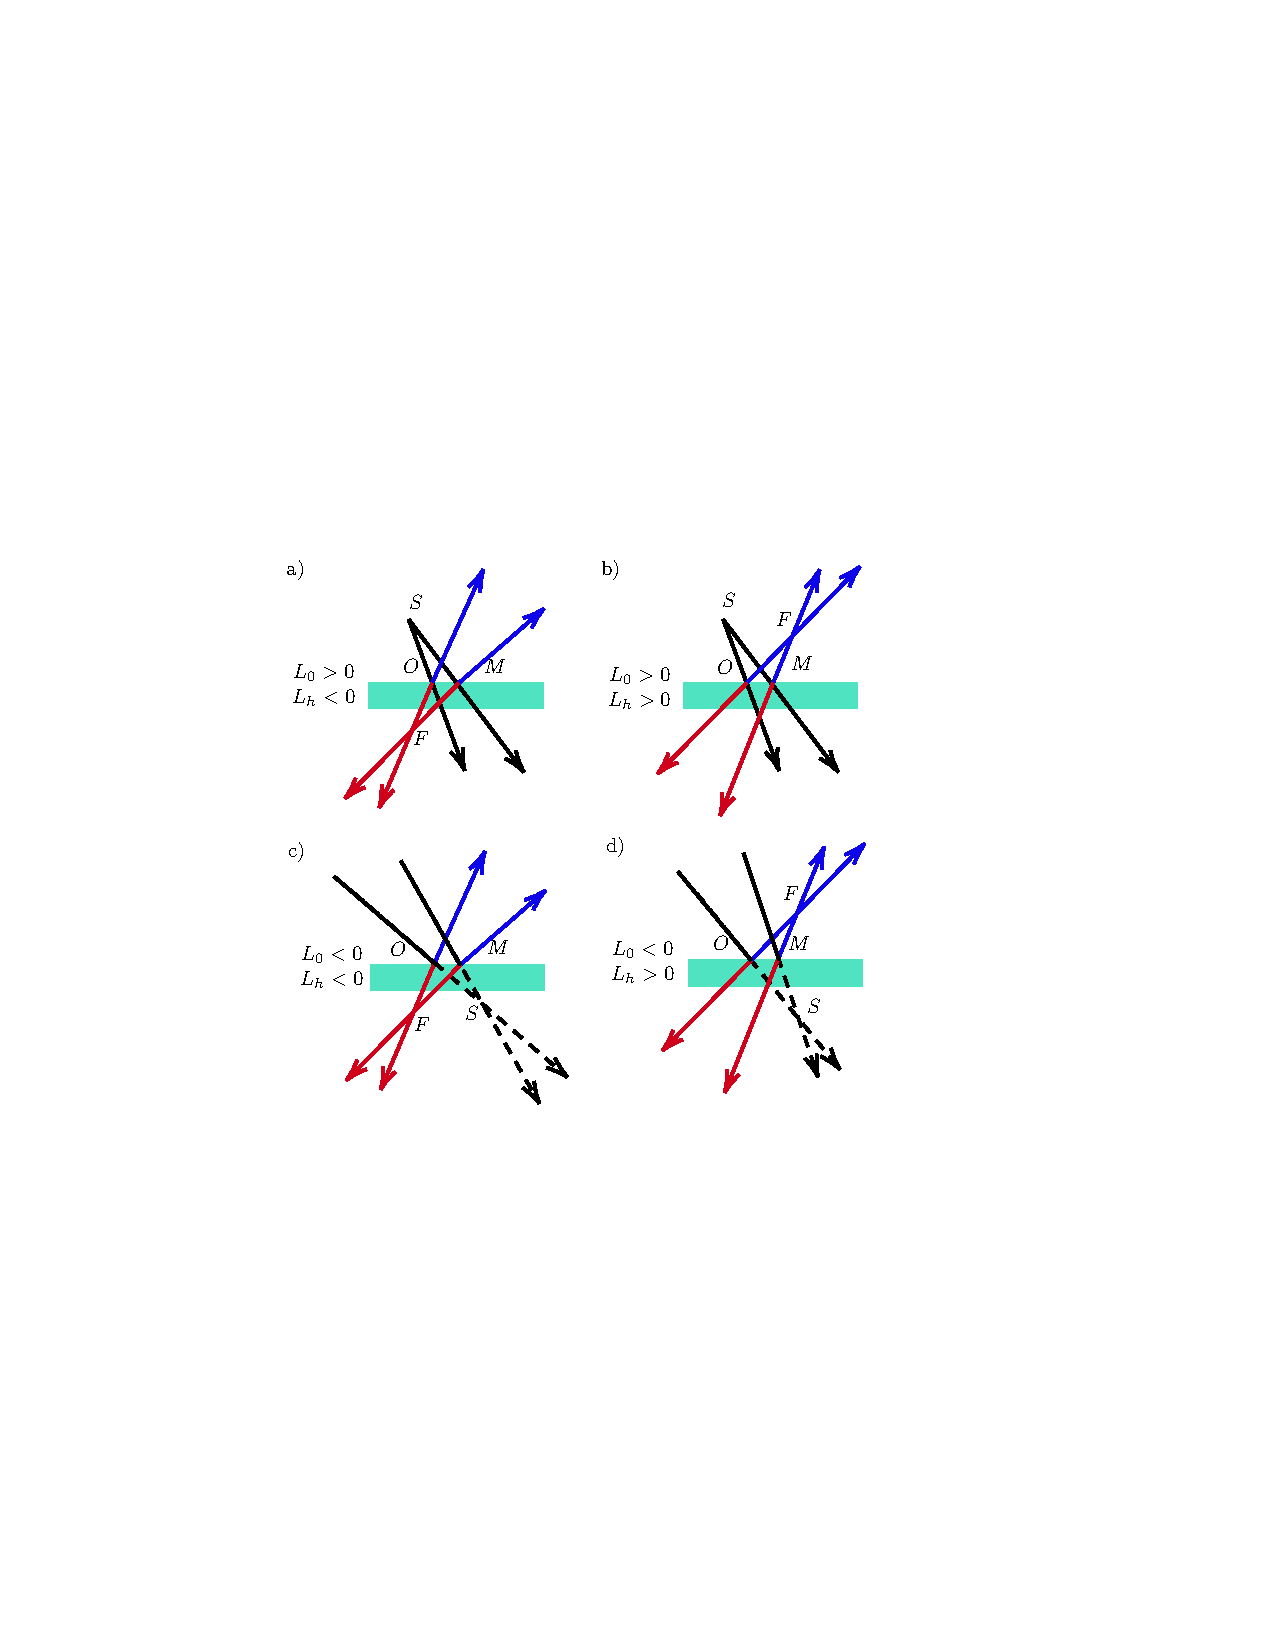
\includegraphics{fig1}
% \end{figure}


\end{document}                    % DO NOT DELETE THIS LINE
%%%%%%%%%%%%%%%%%%%%%%%%%%%%%%%%%%%%%%%%%%%%%%%%%%%%%%%%%%%%%%%%%%%%%%%%%%%%%%
